% =============================================================================
% content.tex -- body of the article (ReScience C template).
% Text produced by \todo{...} is printed in red: it marks information that only
% the author can supply. Fill it in (or delete it) before submitting.
% =============================================================================
\newcommand{\sci}[2]{\ensuremath{#1\times10^{#2}}}
\newcommand{\todo}[1]{\textcolor{darkred}{[\textbf{To do:} #1]}}
\newcommand{\code}[1]{\texttt{#1}}

\section{Introduction}

Neural networks are increasingly used as material models inside gradient-based
topology optimization, where the derivative of the network output with respect
to its inputs enters the sensitivity analysis. Najmon and
Tovar\supercite{Najmon:2024} compared four ways of computing this derivative
for a trained multilayer perceptron (MLP): the analytic chain rule through the
network (the neural network Jacobian, NNJ), central finite differences (CFD),
the complex-step method (CSM)\supercite{Squire:1998,Martins:2003} and automatic
differentiation (AD)\supercite{Baydin:2018}. Each method was used in two
compliance problems on a half MBB beam: density-based topology optimization
(DBTO), in which an MLP replaces the SIMP interpolation of Young's
modulus\supercite{Bendsoe:1989}, and homogenization-based topology optimization
(HBTO)\supercite{Bendsoe:1988}, in which an MLP maps the size of a rectangular
hole in a periodic cell to the homogenized stiffness tensor. The authors
concluded that (i) NNJ, CSM and AD give identical derivatives to working
precision; (ii) CFD is slightly less accurate because of its finite step;
(iii) NNJ and AD are the most consistent methods and are recommended; and
(iv) network-based sensitivities are accurate enough for both problems.

The authors released their code, trained networks, training data and result
files\supercite{NajmonCode}. This article reports an independent replication.
We re-implemented the finite-element analysis, the optimizers, the four
derivative methods and the homogenization in Python, evaluated the authors'
trained networks directly from their files, and also ran the authors' own
functions unchanged. The original study had no reference solution for the HBTO
problem, a limitation its authors point out, and made one optimization run per
method. We therefore added a mesh-converged homogenization model as a reference
and repeated optimization runs to measure their spread.

Every number in the original article that can be recomputed from the released
networks and designs is reproduced (Table~\ref{tab:summary}), and conclusion
(i) holds. Conclusions (ii)--(iv) do not survive the additional checks. The CFD
discrepancy is caused by single-precision rounding of the finite-difference
step in the implementation, not by the method. On the DBTO problem the ranking
of the methods lies within the spread of runs that differ only by round-off.
On the HBTO problem the network's own derivative error is about 600 times
larger, in mean squared error, than the differences between the derivative
methods, and the true compliances of the published HBTO designs are
8.5--10.3\,\% higher than reported. In additional experiments
(Section~\ref{sec:extra}), a network trained on mesh-converged data with
derivative labels gives designs whose true compliance is 3.9--4.6\,\% lower
than that of the best published design.

\begin{table}[htb]
\footnotesize\sffamily
\caption{Results of the original article and their replication. Table, figure
and section numbers in the first column refer to the original article.}
\label{tab:summary}
\begin{tabularx}{\linewidth}{@{}>{\raggedright\arraybackslash}p{2.75cm}%
>{\raggedright\arraybackslash}p{2.35cm}%
>{\raggedright\arraybackslash}X%
>{\raggedright\arraybackslash}p{2.25cm}@{}}
\toprule
Original result & Original value & This replication & Outcome\\
\midrule
DBTO network test error (Table 1) & MSE \sci{1.87}{-7}
  & \sci{1.866}{-7} against the exact SIMP law & Reproduced\\
HBTO network test error (Table 1) & MSE \sci{1.47}{-3}
  & \sci{1.468}{-3} on the authors' test rows & Reproduced\\
NNJ, CSM and AD agree (Secs.~4.2, 4.3) & ``working precision''
  & largest relative difference \sci{7.5}{-16} to \sci{1.5}{-15} & Reproduced\\
CFD differs from NNJ (Figs.~8, 11) & MSE \sci{1.11}{-3} (DBTO), \sci{1.07}{-4} (HBTO)
  & same values, predicted exactly by single-precision rounding of the step
  & Reproduced; cause is the implementation\\
Differences between designs and sensitivities (Figs.~8, 11) & 10 DBTO and 6 HBTO pairs
  & all values to three significant figures & Reproduced\\
DBTO compliance, one run per method (Fig.~5) & 80.84--82.69
  & same values from the saved designs; repeated runs of every method split into
    two groups, near 80.8 and 82.0 & Values reproduced; ranking not supported\\
HBTO compliance (Fig.~9) & 75.70--76.78
  & same values from the network; 82.11--84.72 with converged material models
  & Values reproduced; 8.5--10.3\,\% too low\\
Cost of the methods (Table 2) & CSM cheapest, NNJ and AD most expensive;
  stated as not definitive
  & order depends on the implementation; 1--60\,ms for every method when vectorized
  & Confirms the authors' caveat\\
Worked example (Appendix B) & 1.623
  & 1.623; three sign typos in intermediate vectors & Reproduced\\
\midrule
Not replicated & \multicolumn{3}{>{\raggedright\arraybackslash}p{9.9cm}@{}}{training times;
  the 100-sample DBTO network of Fig.~6 (not in the repository); iteration counts
  of the authors' HBTO runs, which take 30--36\,h each with their optimizer}\\
\bottomrule
\end{tabularx}
\end{table}

\section{Methods}

\subsection{The original study}
Both problems use a $60\times30$ mesh of bilinear elements on a half MBB beam,
a volume fraction of 0.5, a sensitivity filter of radius
2.7 elements\supercite{Sigmund:2001,Sigmund:1998}, and SciPy's
\code{trust-constr} optimizer\supercite{Virtanen:2020} with a tolerance of
$10^{-3}$. In DBTO a 1--64--1 MLP with sigmoid hidden units replaces the SIMP
law $E(\theta)=E_\mathrm{min}+(E_0-E_\mathrm{min})\,\theta^{p}$ with $E_0=1$,
$E_\mathrm{min}=10^{-9}$ and $p=3$, which therefore serves as an exact
reference. In HBTO each element has two design variables, the width $\theta_1$
and the height $\theta_2$ of a rectangular hole in a square cell, and a
2--64--4 sigmoid MLP (452 parameters) returns the homogenized tensor entries
$(C_{11},C_{12},C_{22},C_{66})$. Both networks were trained with Adam for
5\,000 epochs on 10\,000 Latin-hypercube samples, split 70/15/15 into training,
validation and test sets; the HBTO samples were homogenized on a $100\times100$
voxel grid. The derivative methods use $h=10^{-6}$ (CFD), $h=10^{-12}$ (CSM)
and TensorFlow gradient tapes\supercite{Abadi:2016} (AD). The article reports
one optimization run per method and problem.

\subsection{Replication code}
The replication is a Python package written for this study (\code{nnto}), built
on NumPy and SciPy\supercite{Harris:2020,Virtanen:2020}; it does not need
TensorFlow. It contains
\begin{itemize}
\item a reader for the authors' TensorFlow checkpoint files, so that the
  published networks themselves are evaluated;
\item vectorized finite-element analysis, sensitivity and density
  filters\supercite{Andreassen:2011,Bourdin:2001,Bruns:2001}, and drivers for
  SciPy's \code{trust-constr}, the optimality criteria and
  MMA\supercite{Svanberg:1987}, in which every peculiarity of the original code
  is a named option, so that the original behaviour remains available as a
  baseline;
\item the four derivative methods, with forward- and reverse-mode AD from a
  small engine written for the package, and second derivatives;
\item voxel homogenization, which regenerates the authors' HBTO data set, and
  body-fitted homogenization with exact derivatives with respect to the hole
  size\supercite{Andreassen:2014};
\item 107 unit tests, several of which reproduce numbers stored in the
  authors' result files.
\end{itemize}
The authors' scripts start training or optimization as soon as they are
imported, and they need TensorFlow. To run their code as well, the package
compiles the functions defined in the original scripts, without changing any
line, and executes them with a small NumPy stand-in for the Keras calls they
make. This reproduces the numbers saved by the authors to 6--11 significant
digits.

\subsection{Reference models}\label{sec:reference}
For DBTO the exact SIMP law and its derivative are the reference. For HBTO we
computed the homogenized tensor of the rectangular-hole cell with body-fitted
finite elements at two mesh refinements, extrapolated the results to mesh
convergence (Richardson extrapolation), and tabulated the values and their
exact derivatives with respect to $(\theta_1,\theta_2)$ on a $51\times51$ grid
over $[0.01,0.99]^2$. A bicubic spline of this table is the reference material
model. At 300 independent Latin-hypercube points it agrees with direct
converged computations to a relative $L_2$ difference of \sci{5.6}{-5} in the
tensor entries and 0.7\,\% in their derivatives. These 300 points are the test
set for every network in this article.

Holes with a side below 0.01 need a convention. In the authors' voxel data a
hole narrower than one voxel disappears, so such cells are solid; the
converged reference, tabulated from 0.01 upwards, would instead treat them as
1\,\% slits, which are much softer. We report both. The \emph{true compliance}
of a design is its compliance evaluated with a reference model, as opposed to
the compliance predicted by the network that produced it.

\subsection{Repeated runs and statistics}\label{sec:noise}
Optimization paths are sensitive to round-off. To measure the spread that this
alone produces, DBTO runs were repeated from the same starting design with the
gradient multiplied element-wise by $1+\epsilon\xi$, where $\xi$ is a standard
normal random number and $\epsilon=10^{-10}$, using different random seeds.
Repeated results are reported as mean $\pm$ 95\,\% confidence half-width
(Student's $t$), and configurations are compared with Welch's $t$-test.

\subsection{Computing environment and reproducibility}
The results were first produced on the author's computer (macOS) and then
re-run from scratch on Linux (Python 3.13.18, NumPy 2.5.3, SciPy 1.18.1, two
cores, about two hours of computation). Only the long DBTO noise-floor
ensembles were not re-run; the repeated runs of Section~\ref{sec:dbto} answer
the same question and were re-run. Deterministic results are identical
between the two runs: the reference model, the accuracy of all 60 retrained
networks of Section~\ref{sec:extra} and all 31 optimization runs of that
section. Three kinds of results differ between the machines without changing
any conclusion: round-off-sized numbers (below $10^{-9}$), which vary by up to a
factor of two; the chaotic DBTO optimization paths
(Section~\ref{sec:dbto}); and timings. Table~\ref{tab:scripts} lists the
scripts behind each result; the repository README gives the commands.

\begin{table}[htb]
\footnotesize\sffamily
\caption{Scripts (folder \code{experiments/} of the code repository) that
produce each result.}
\label{tab:scripts}
\begin{tabularx}{\linewidth}{@{}>{\raggedright\arraybackslash}p{3.6cm}%
>{\raggedright\arraybackslash}X@{}}
\toprule
Result & Scripts\\
\midrule
Reference models (Sec.~\ref{sec:reference}) & \code{gt\_voxel\_lattice.py},
  \code{gt\_fitted\_grid.py}, \code{gt\_offgrid.py}\\
Sec.~\ref{sec:agree}, Table~\ref{tab:methods}, Fig.~\ref{fig:cfd}
  & \code{exp\_surrogate\_truth.py}, \code{exp\_precision.py},
  \code{exp\_higher\_order.py}, \code{exp\_architectures.py}\\
Sec.~\ref{sec:dbto}, Fig.~\ref{fig:dbto} & \code{exp\_patch\_check.py},
  \code{analyse\_patch\_check.py}, \code{exp\_dbto\_ensemble.py},
  \code{exp\_dbto\_part2.py}\\
Sec.~\ref{sec:hbto}, Table~\ref{tab:hbto}, Figs.~\ref{fig:hbto}--\ref{fig:jac}
  & \code{exp\_surrogate\_truth.py}, \code{rescore\_final\_designs.py}\\
Sec.~\ref{sec:cost} & \code{exp\_efficiency.py}\\
Sec.~\ref{sec:discrepancies}, Table~\ref{tab:discrepancies}
  & unit tests in \code{tests/}, \code{exp\_audit\_extras.py}\\
Sec.~\ref{sec:extra}, Tables~\ref{tab:newacc}--\ref{tab:ablation},
  Fig.~\ref{fig:designs} & \code{exp\_newer\_models.py},
  \code{exp\_newer\_models\_to.py}, \code{analyse\_newer\_models.py},
  \code{exp\_published\_long.py}, \code{rescore\_final\_designs.py}\\
Figures & \code{make\_figures.py}, \code{make\_comparison\_figure.py}\\
\bottomrule
\end{tabularx}
\end{table}

\section{Results}

\subsection{Network accuracy and agreement of NNJ, CSM and AD}\label{sec:agree}
The published DBTO network differs from the exact SIMP law by a mean squared
error (MSE) of \sci{1.866}{-7}, and the HBTO network reaches an MSE of
\sci{1.468}{-3} on the authors' test rows, as in Table~1 of the original
article (\sci{1.87}{-7} and \sci{1.47}{-3}). In double precision, CSM and
forward- and reverse-mode AD agree with NNJ to a largest relative difference
between \sci{7.5}{-16} and \sci{1.5}{-15} for both networks
(Table~\ref{tab:methods}). The same holds for second derivatives (the analytic
Hessian, hyper-dual AD and the complex step of the Jacobian agree to
\sci{3}{-15}), and in a one-dimensional study of six architectures, including
residual, Fourier-feature and ReLU networks, CSM and AD agree with NNJ to
\sci{4}{-15} or better. Conclusion (i) therefore holds and extends beyond the
networks of the original study, with two caveats: CFD fails near the kinks of
ReLU networks, and CSM needs access to the network weights, because the
forward pass has to be re-implemented with complex numbers. The latter
contradicts the original article's suggestion to use CFD and CSM for
third-party networks whose details are not accessible.

\begin{table}[htb]
\footnotesize\sffamily
\caption{Largest difference from the double-precision NNJ derivative over
4\,000 random inputs, relative to the largest magnitude of the same derivative
entry. ``Float32 inputs'' is the published CFD implementation.}
\label{tab:methods}
\begin{tabularx}{\linewidth}{@{}>{\raggedright\arraybackslash}X%
>{\raggedleft\arraybackslash}p{2.0cm}>{\raggedleft\arraybackslash}p{2.0cm}@{}}
\toprule
Method and precision & DBTO & HBTO\\
\midrule
AD, forward mode, float64 & \sci{7.5}{-16} & \sci{8.0}{-16}\\
AD, reverse mode, float64 & \sci{8.9}{-16} & \sci{1.3}{-15}\\
CSM, $h=10^{-12}$, complex128 & \sci{1.0}{-15} & \sci{1.5}{-15}\\
CFD, $h=10^{-6}$, float64 & \sci{2.3}{-10} & \sci{1.1}{-9}\\
CFD, $h=10^{-6}$, float32 inputs (as published) & \sci{1.65}{-2} & \sci{1.53}{-2}\\
CFD, $h=10^{-6}$, float32 inputs, divided by the step actually taken
  & \sci{3.1}{-8} & \sci{4.2}{-8}\\
NNJ, float32 & \sci{2.8}{-7} & \sci{7.0}{-7}\\
AD, reverse mode, float32 & \sci{3.5}{-7} & \sci{7.0}{-7}\\
CSM, $h=10^{-12}$, complex64 & \sci{4.1}{-7} & \sci{7.1}{-7}\\
\bottomrule
\end{tabularx}
\end{table}

\subsection{The CFD discrepancy is a single-precision artefact}\label{sec:cfd}
The original article finds that CFD differs from the other three methods, with
an MSE between the CFD and NNJ sensitivities of \sci{1.11}{-3} for DBTO
(Fig.~8) and \sci{1.07}{-4} for HBTO (Fig.~11), and attributes this to the
finite step. We obtain the same two values, and they are explained exactly by
the precision of the implementation. The optimization scripts load the networks
without setting Keras' floating-point type to double precision, unlike the
authors' training and example scripts, and \code{Model.predict} then receives
the perturbed inputs $\theta\pm h$ rounded to single
precision\supercite{IEEE754:2019}. For $\theta\in[0.5,1)$ the spacing of
single-precision numbers is $2^{-24}\approx\sci{5.96}{-8}$, so the step
$2h=\sci{2}{-6}$ by which the code divides is 33.55 spacings, whereas the
rounded inputs differ by 33 or 34 spacings. Depending on $\theta$, every CFD
derivative is therefore scaled by a factor between 0.9835 and 1.0133, an error
of $-1.65$ to $+1.33\,\%$. At the uniform starting designs the factor is
1.0133 for every element: the ratio of the CFD to the NNJ sensitivities stored
in the authors' result files is 1.0133 with a standard deviation of
\sci{7.7}{-10} (DBTO) and \sci{5.0}{-8} (HBTO), and an MSE computed from this
single factor reproduces both published values. Along an optimization path the
published CFD sensitivities stay 1.3--1.7\,\% wrong.

In double precision, CFD with the same step agrees with NNJ to \sci{2.3}{-10}
(DBTO) and \sci{1.1}{-9} (HBTO) (Fig.~\ref{fig:cfd}, Table~\ref{tab:methods}).
The fix is a single line before the networks are loaded:
\begin{center}
\code{tf.keras.backend.set\_floatx('float64')}
\end{center}
We could not run TensorFlow itself: the rounding is
inferred from the authors' stored results, which match a model of
single-precision input rounding to the digits given above. The repository
script \code{tf\_crosscheck\_float32.py} checks it with TensorFlow.

\begin{figure}[htb]
\centering
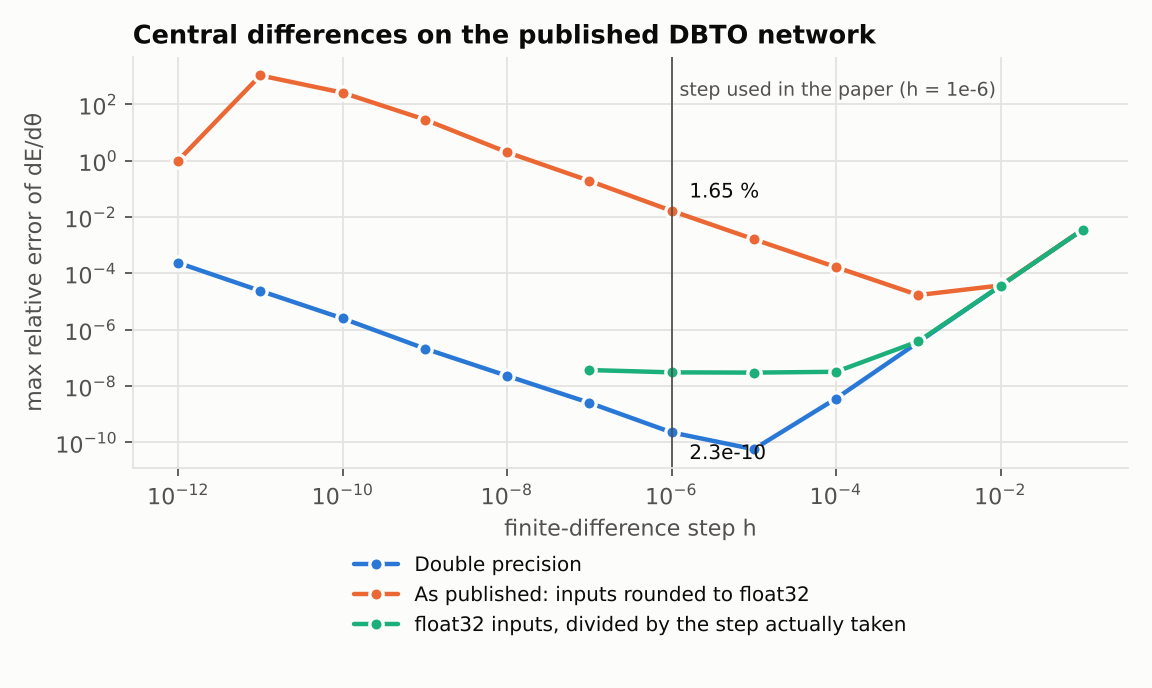
\includegraphics[width=0.92\linewidth]{figures/fig1_cfd_step.png}
\caption{Largest relative error of central differences on the published DBTO
network over 4\,000 random inputs, as a function of the step $h$. Blue: double
precision. Orange: inputs rounded to single precision, as in the published
implementation (1.65\,\% at the step used in the original article). Green: the
same rounded inputs, divided by the step actually taken.}
\label{fig:cfd}
\end{figure}

\subsection{Density-based optimization: the ranking of methods is within run-to-run noise}\label{sec:dbto}
Evaluated with the material model that produced them, the authors' five saved
DBTO designs give exactly the compliances printed in Fig.~5 of the original
article (80.84 to 82.69), and the compliances of the four network-based designs
under the exact SIMP law differ from these by at most 0.1\,\%. The ten design
differences and ten sensitivity differences of Fig.~8 are reproduced to three
significant figures. The network error is therefore not an issue for DBTO.

The ranking of the methods is another matter. The original article already
attributes the differences between the NNJ, CSM and AD runs, whose
sensitivities are identical, to accumulated numerical errors. Repeated runs show
how large these differences are. Runs that start from the same design and
differ only by gradient perturbations of relative size $10^{-10}$ end in two
groups of designs about 1.5\,\% apart (Fig.~\ref{fig:dbto}). On the author's
computer, eight of ten runs with published or corrected CFD and NNJ
sensitivities reached true compliances of 80.77--80.88 and two reached
82.06--82.16; on Linux, 19 runs gave 80.72--81.03 and 81.94--82.12. Runs with
the exact SIMP law also land in both groups. Which group a run reaches is
decided by round-off, not by the derivative method. The differences between
the methods in the original Fig.~5 are of the same size as the spread between
runs of a single method, and the highest value there, CSM (82.69), comes from a
run that stopped because its trust region collapsed
(Table~\ref{tab:discrepancies}). A ranking of the methods from one run each is
therefore not supported.

Correcting the CFD step changes the path but not the outcome. Measured against
a run with exact derivatives, the published CFD run leaves the path (largest
design difference above $10^{-3}$) at iteration 3 and the corrected one at
iteration 71. Over six runs each, the mean true compliance is
$81.03\pm0.57$ with the published CFD and $81.20\pm0.67$ with the corrected CFD
(Welch $p=0.63$). Our runs take 220--405 iterations, against 287--657 in the
original article; they used SciPy 1.18 instead of 1.10, and the
\code{trust-constr} paths leave the authors' logged paths after six iterations.

\begin{figure}[htb]
\centering
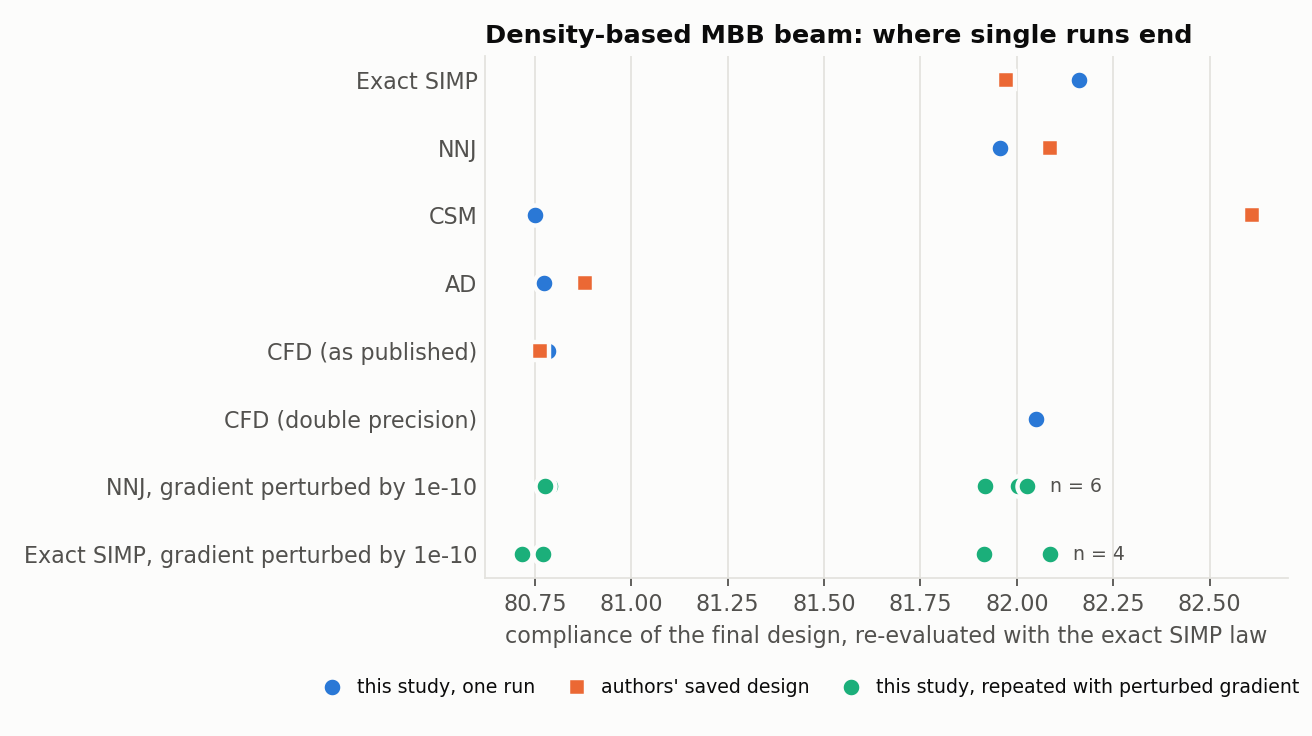
\includegraphics[width=\linewidth]{figures/fig2_dbto_runs.png}
\caption{True compliance (exact SIMP law) of final DBTO designs. Squares: the
authors' saved designs. Blue circles: one run per configuration in this study.
Green circles: runs repeated with the gradient perturbed by a relative
$10^{-10}$ (six runs with NNJ, four with the exact SIMP law). Whatever the
derivative, the runs of this study end in one of two groups, near 80.8 and
near 82.}
\label{fig:dbto}
\end{figure}

\subsection{Homogenization-based optimization: the network error dominates}\label{sec:hbto}
Evaluated with the authors' network, the four saved HBTO designs give exactly
the compliances printed in Fig.~9 of the original article, and the six design
differences of Fig.~11 are reproduced once the 7.5\,\% thresholding mentioned
in the caption of Fig.~9 is applied. Evaluated with material models that do
not come from the network, the same designs are 8.5--10.3\,\% less stiff than
reported (Table~\ref{tab:hbto}, Fig.~\ref{fig:hbto}). The authors' own voxel
model, which generated their training data, gives 8.5--9.7\,\%. The converged
reference gives the same range when holes narrower than 1\,\% count as solid,
as in the training data, and 9.2--10.3\,\% when they count as thin slits.
About 30\,\% of the cells of these designs have a hole side below 0.01.

\begin{table}[htb]
\footnotesize\sffamily
\caption{Compliance of the authors' four final HBTO designs: as reported
(evaluated by the network) and evaluated with independent material models.
Last column: how much higher the independent values are than the reported one.}
\label{tab:hbto}
\begin{tabularx}{\linewidth}{@{}l*{4}{>{\raggedleft\arraybackslash}X}%
>{\raggedleft\arraybackslash}p{1.9cm}@{}}
\toprule
 & Reported & Voxel model & Converged, holes ${<}1\,\%$ solid
 & Converged, thin slits & Higher than reported\\
\midrule
NNJ & 75.70 & 82.16 & 82.11 & 82.65 & 8.5--9.2\,\%\\
CFD & 76.78 & 84.25 & 84.21 & 84.72 & 9.7--10.3\,\%\\
CSM & 76.14 & 82.59 & 82.59 & 83.16 & 8.5--9.2\,\%\\
AD  & 75.70 & 82.36 & 82.32 & 82.80 & 8.7--9.4\,\%\\
\bottomrule
\end{tabularx}
\end{table}

The cause is the network, not the derivative method. Against the converged
reference at the 300 test points, the published network has a relative RMS
error of 4.1\,\% in the tensor entries and 64\,\% in their derivatives
(14\,\% in the interior $[0.1,0.9]^2$), and 1.9\,\% of its predictions are not
positive definite. The derivative error is largest near the edges of the
parameter domain (Fig.~\ref{fig:jac}), where the training targets jump because
the voxel data label holes narrower than one voxel as solid, and where many
cells of the optimized designs lie. At the uniform starting design the network
underestimates the compliance by 8.8\,\% (255.61 against 280.19), and its
sensitivities differ from the true ones by 22\,\% in relative $L_2$ norm, or
25\,\% after the sensitivity filter. The difference between CFD and NNJ
reported in Fig.~11 of the original article, an MSE of \sci{1.07}{-4} on the
filtered sensitivities, is 601 times smaller than the error that all four
methods share on the same basis, an MSE of \sci{6.4}{-2}; in relative $L_2$
norm it is 19 times smaller (1.3\,\% against 25\,\%). For the authors' best
design the network's prediction of the compliance is 7.8--8.4\,\% too low.

\begin{figure}[htb]
\centering
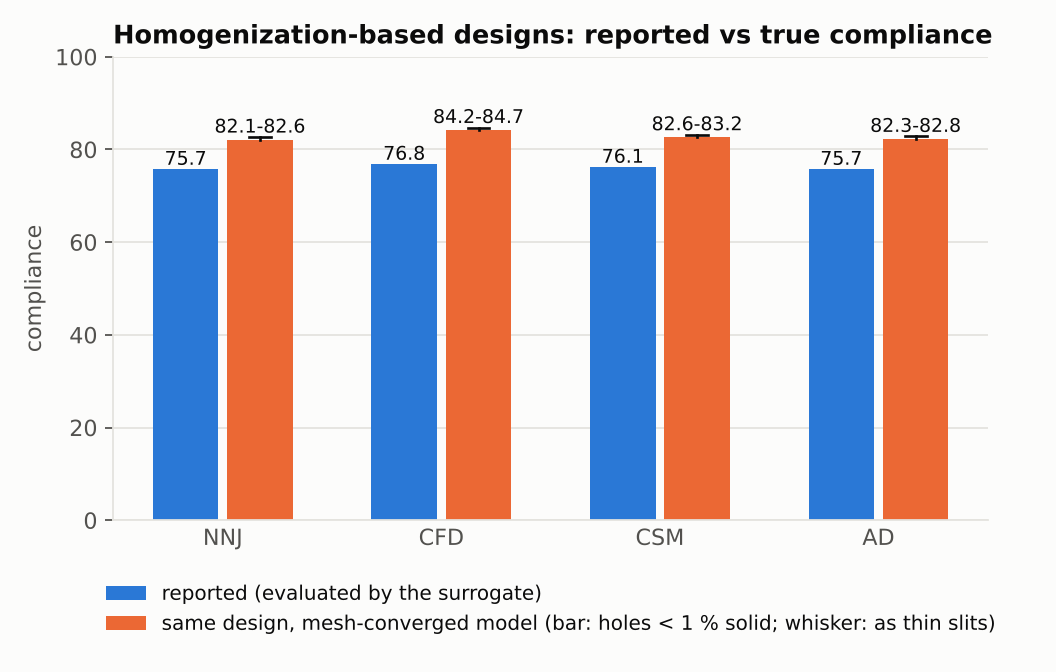
\includegraphics[width=0.85\linewidth]{figures/fig3_hbto_reported_vs_true.png}
\caption{Compliance of the authors' four HBTO designs as reported (evaluated by
the network) and evaluated with the converged reference (bars: holes narrower
than 1\,\% counted as solid; whiskers: counted as thin slits).}
\label{fig:hbto}
\end{figure}

\begin{figure}[htb]
\centering
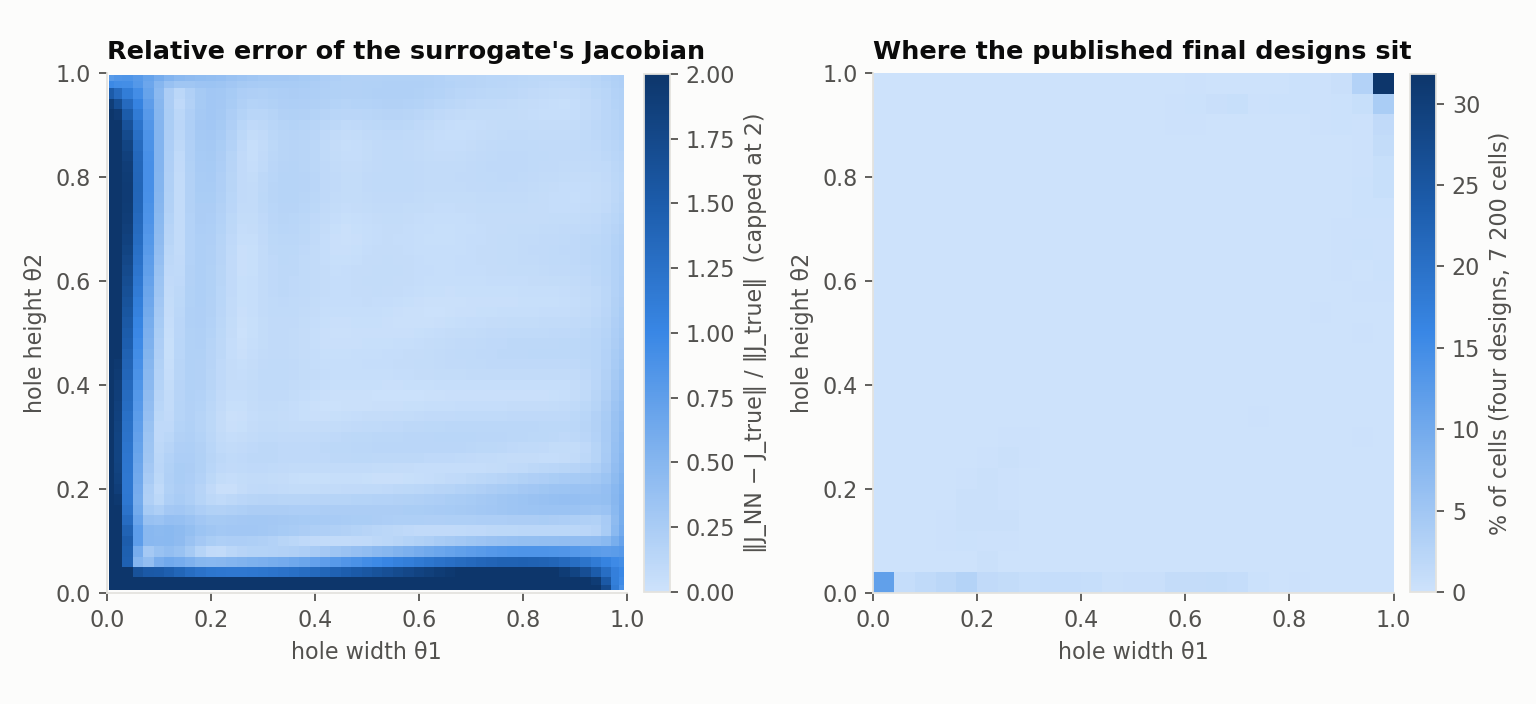
\includegraphics[width=\linewidth]{figures/fig4_hbto_jacobian_error.png}
\caption{Left: relative error of the Jacobian of the published HBTO network
against the converged reference, capped at 2. Right: share of the cells of the
authors' four final designs in each part of the $(\theta_1,\theta_2)$ plane.}
\label{fig:jac}
\end{figure}

\subsection{Computational cost}\label{sec:cost}
Table~2 of the original article ranks CSM as the cheapest method (0.088\,s and
0.180\,s per sensitivity evaluation for DBTO and HBTO) and NNJ and AD as the
most expensive (2.6--8.6\,s), and cautions that the implementations were not
optimized, so that the times are not definitive. Our measurements support this
caveat. The original routines, run without TensorFlow on
the 1\,800 elements of the mesh, give a different order on the author's
computer: CFD 2--4\,ms, CSM 0.11--0.23\,s, NNJ 0.14--0.16\,s and AD
1.1--5.9\,s (up to about four times faster, in the same order, in the Linux rerun). The order reflects the
implementations: NNJ loops over the elements in Python, and the AD routine
builds the full Jacobian of all outputs with respect to all inputs across the
batch (207\,MB for HBTO, where the per-element Jacobians need 115\,kB).
Vectorized, all five routines, including forward- and reverse-mode AD, take
1--60\,ms. In either form the derivatives are a small part of an optimization
iteration, whose cost is dominated by the dense constraint Jacobian passed to
\code{trust-constr}: with a sparse Jacobian an iteration on the $60\times30$
mesh was 111--174 times faster on the machines we used, with the same iterates
to round-off. The timings in Table~2 of the original article therefore
characterize the implementations rather than the methods. When a scalar
function of many inputs is differentiated, only reverse-mode AD stays cheap.

\subsection{Differences between the article and the code}\label{sec:discrepancies}
Table~\ref{tab:discrepancies} lists the differences between the article and
the code that we found while replicating; each is checked by a unit test. The
code is correct where the article's equations are wrong, so none of these
changes the published numbers, but several make the article hard to follow or
the results hard to reproduce.

\begin{table}[htb]
\footnotesize\sffamily
\caption{Differences between the original article and the original code, and
problems in the code. ``Code'' refers to the published repository.}
\label{tab:discrepancies}
\begin{tabularx}{\linewidth}{@{}>{\raggedright\arraybackslash}p{2.3cm}%
>{\raggedright\arraybackslash}X%
>{\raggedright\arraybackslash}p{3.2cm}@{}}
\toprule
Where & Finding & Consequence\\
\midrule
Eq.~(11) & Printed as $+\mathbf{u}^\mathsf{T}(\partial\mathbf{K}/\partial\theta_e)\mathbf{u}$;
  the derivative of compliance is $-\mathbf{u}^\mathsf{T}(\partial\mathbf{K}/\partial\theta_e)\mathbf{u}$.
  The code is correct. & None on results\\
Eq.~(15) & Printed as $-p(E_0-E_\mathrm{min})\theta^{p-1}$; the derivative of the
  SIMP law is positive. The code is correct. & Used together, the two printed
  signs cancel for SIMP but not for a network derivative\\
Eqs.~(1)--(6) & A layer is written $F(\mathbf{W}\mathbf{y}+\mathbf{B})$, but
  Eqs.~(3)--(6) are only valid for row vectors, $F(\mathbf{y}\mathbf{W}+\mathbf{B})$,
  as in Appendix B and the code & Factors not conformable as printed\\
Sec.~4.2, Fig.~4(a) & A cantilever (clamped left edge) is described; the code
  and the published topologies use a half MBB beam & None on results\\
Appendix B & Sign typos in the intermediate vectors (B15b), (B16c) and (B18b);
  the final value 1.623 is correct & None on results\\
Stopping rule & The article stops when the largest change in $\theta$ is below
  $10^{-3}$; in the code the tolerance sets \code{xtol}, \code{gtol} and
  \code{barrier\_tol}, and the DBTO-CSM run and three HBTO runs stop because the
  trust region collapses & Iteration counts partly measure trust-region collapse\\
Sensitivity filter & The heuristically filtered sensitivities are passed to
  \code{trust-constr} as the gradient; their cosine with the true gradient at
  the final designs is 0.86 (DBTO) and 0.17--0.21 (HBTO) & Gradient
  inconsistent with the objective\\
Clipping & Network predictions are clipped, but their derivatives are not set to
  zero where clipping applies (21.6--25.5\,\% of the cells of the HBTO designs)
  & Gradient inconsistent with the objective\\
Volume constraint & The Jacobian of the DBTO volume constraint is 1\,800 times
  too large & Constraint scaling only\\
Training scripts & Early stopping is defined but not used; the validation split
  does not select the model; inputs are normalized with training and
  validation data & Minor\\
Repository & The 100-sample DBTO network of Fig.~6 is missing;
  \code{Run\_HBTO\_NN.py} ships with \code{maxiter = 50} and the CFD method
  selected & Fig.~6 cannot be reproduced; settings must be edited\\
\bottomrule
\end{tabularx}
\end{table}

\FloatBarrier
\section{Beyond the replication: a better HBTO network}\label{sec:extra}
Since the network error dominates the HBTO results, we asked how much better
the designs become with a better network, and which change is responsible.
This section goes beyond the original article.

\subsubsection{Setup} All runs use one formulation, so that differences come from
the material model: a density-type filter on both hole fields with the exact
chain rule, an exact volume-constraint Jacobian, double precision, hole sizes
in $[0.01,0.99]$, derivatives set to zero wherever a prediction is clipped,
and MMA\supercite{Svanberg:1987} with a move limit of 0.2 until the largest
design change falls below $10^{-3}$ or 3\,000 iterations are reached. Every
final design is scored with the converged reference. Optimizing with the
reference model itself gives the \emph{reference optimum}, 78.853 (four runs,
identical to three decimals). Six architectures were trained, with
hyperparameters fixed in advance: the original 1$\times$64 sigmoid MLP, a
3$\times$64 tanh MLP, a residual network (4$\times$64,
swish)\supercite{He:2016}, a Fourier-feature network (16 features, 2$\times$64
tanh)\supercite{Tancik:2020}, a SIREN (3$\times$64)\supercite{Sitzmann:2020}
and a Kolmogorov--Arnold network\supercite{Liu:2025} with Chebyshev edge
functions (2--16--16--4). Each was trained with L-BFGS for 2\,000 iterations on
(a) the authors' data, (b) the 2\,601 values of the converged $51\times51$
table, or (c) the same table with its exact derivatives as additional labels
(Sobolev training\supercite{Czarnecki:2017}); variant (c) was also combined
with an output head that writes the tensor as $\mathbf{L}\mathbf{L}^\mathsf{T}$,
which is always positive definite. Every configuration was trained with three
seeds, and each trained network was used in one optimization run (two for the
architecture comparison).

\begin{table}[htb]
\footnotesize\sffamily
\caption{Accuracy of the published HBTO network and of the 3$\times$64 tanh MLP
trained on converged data with derivative labels, at the 300 test points.
Positive definiteness is checked on a $197\times197$ grid.}
\label{tab:newacc}
\begin{tabularx}{\linewidth}{@{}>{\raggedright\arraybackslash}X%
>{\raggedleft\arraybackslash}p{2.4cm}>{\raggedleft\arraybackslash}p{3.2cm}@{}}
\toprule
 & Published network & 3$\times$64 tanh, converged data + derivative labels\\
\midrule
Relative RMS error, tensor entries & 4.1\,\% & 0.025\,\%\\
Relative RMS error, derivatives (all / interior) & 64\,\% / 14\,\% & 0.51\,\% / 0.28\,\%\\
Predictions not positive definite & 1.9\,\% & 2.1\,\% (0\,\% with $\mathbf{L}\mathbf{L}^\mathsf{T}$ head)\\
Starting design: compliance error / sensitivity error & $-8.8$\,\% / 22\,\% & $+1.0$\,\% / 3.1\,\%\\
Parameters / training time & 452 / -- & 8\,772 / 142\,s\\
\bottomrule
\end{tabularx}
\end{table}

\subsubsection{Results} The 3$\times$64 tanh MLP trained on converged data with
derivative labels reduces the network error by more than two orders of
magnitude (Table~\ref{tab:newacc}). Its designs have a true compliance of
$78.876\pm0.154$ (three runs), between $-0.02$ and $+0.12\,\%$ from the
reference optimum, and the network predicts their compliance to within
0.08\,\% (mean absolute error 0.035\,\%), against 7.8--8.4\,\% for the
authors' best design (Fig.~\ref{fig:designs}). This is 3.9--4.6\,\% below the
true compliance of the best published design: 3.94\,\% when holes narrower
than 1\,\% count as solid, 3.99\,\% under the voxel model and 4.56\,\% when they
count as thin slits.

Part of this gain comes from the formulation and the optimizer, which were
changed together. With the same formulation and MMA, the published network
reaches $81.959\pm0.213$ at the 3\,000-iteration limit without converging,
3.76\,\% above the improved network (difference 3.08, 95\,\% CI 2.91--3.26,
Welch $p=\sci{2.5}{-6}$; 3.66\,\% when both are compared at exactly the target
volume). Continued to 10\,000 iterations it reaches 80.50--80.62 (three runs),
and between 11\,000 and 30\,000 iterations it oscillates between 80.45 and
80.96 without converging. Of the 3.9--4.6\,\% gain over the published designs,
about 2\,\% is therefore due to the network and 1.8--2.6\,\% to the consistent
formulation and optimizer.

No single change accounts for the network's share (Table~\ref{tab:ablation}).
Converged training data, or more capacity, each bring the designs to within
0.3--0.8\,\% of the reference optimum; together they come within 0.12\,\%.
Derivative labels mainly buy convergence: without them the deep MLP reaches
similar designs but does not converge within 3\,000 iterations. The newer
architectures, trained the same way, reach the same designs as the plain deep
MLP (78.83--78.87).

\begin{table}[htb]
\footnotesize\sffamily
\caption{True compliance of the final HBTO designs (mean $\pm$ 95\,\% confidence
half-width over runs; lower is better). All runs use the same formulation and
MMA. ``Converged data'': the $51\times51$ mesh-converged table.}
\label{tab:ablation}
\begin{tabularx}{\linewidth}{@{}>{\raggedright\arraybackslash}X%
>{\raggedleft\arraybackslash}p{2.2cm}>{\centering\arraybackslash}p{0.7cm}%
>{\centering\arraybackslash}p{1.3cm}>{\raggedleft\arraybackslash}p{1.8cm}@{}}
\toprule
Material model & True compliance & Runs & Converged & Iterations\\
\midrule
Reference model (reference optimum) & 78.853 & 4 & yes & 1\,428--1\,554\\
Published network & $81.959\pm0.213$ & 3 & no & 3\,000\\
\midrule
1$\times$64 sigmoid, converged data + derivative labels & $79.305\pm0.239$ & 3 & yes & 623--1\,118\\
3$\times$64 tanh, authors' data & $79.240\pm0.493$ & 3 & no & 3\,000\\
3$\times$64 tanh, converged data, values only & $78.862\pm0.118$ & 3 & no & 3\,000\\
3$\times$64 tanh, converged data + derivative labels & $78.876\pm0.154$ & 3 & yes & 694--1\,148\\
\quad same, $\mathbf{L}\mathbf{L}^\mathsf{T}$ output head & $78.850\pm0.069$ & 2 & yes & 1\,541--1\,823\\
\midrule
Residual 4$\times$64 swish, converged data + labels & $78.847\pm0.022$ & 2 & yes & 1\,267--1\,657\\
Fourier features + 2$\times$64 tanh, converged data + labels & $78.833\pm0.001$ & 2 & yes & 1\,198--1\,378\\
SIREN 3$\times$64, converged data + labels & $78.865\pm0.386$ & 2 & yes & 990--1\,089\\
Chebyshev KAN 2--16--16--4, converged data + labels & $78.844\pm0.076$ & 2 & yes & 1\,340--1\,386\\
\quad same, $\mathbf{L}\mathbf{L}^\mathsf{T}$ output head & $78.954\pm1.254$ & 2 & yes & 892--1\,421\\
\bottomrule
\end{tabularx}
\end{table}

\begin{figure}[htb]
\centering
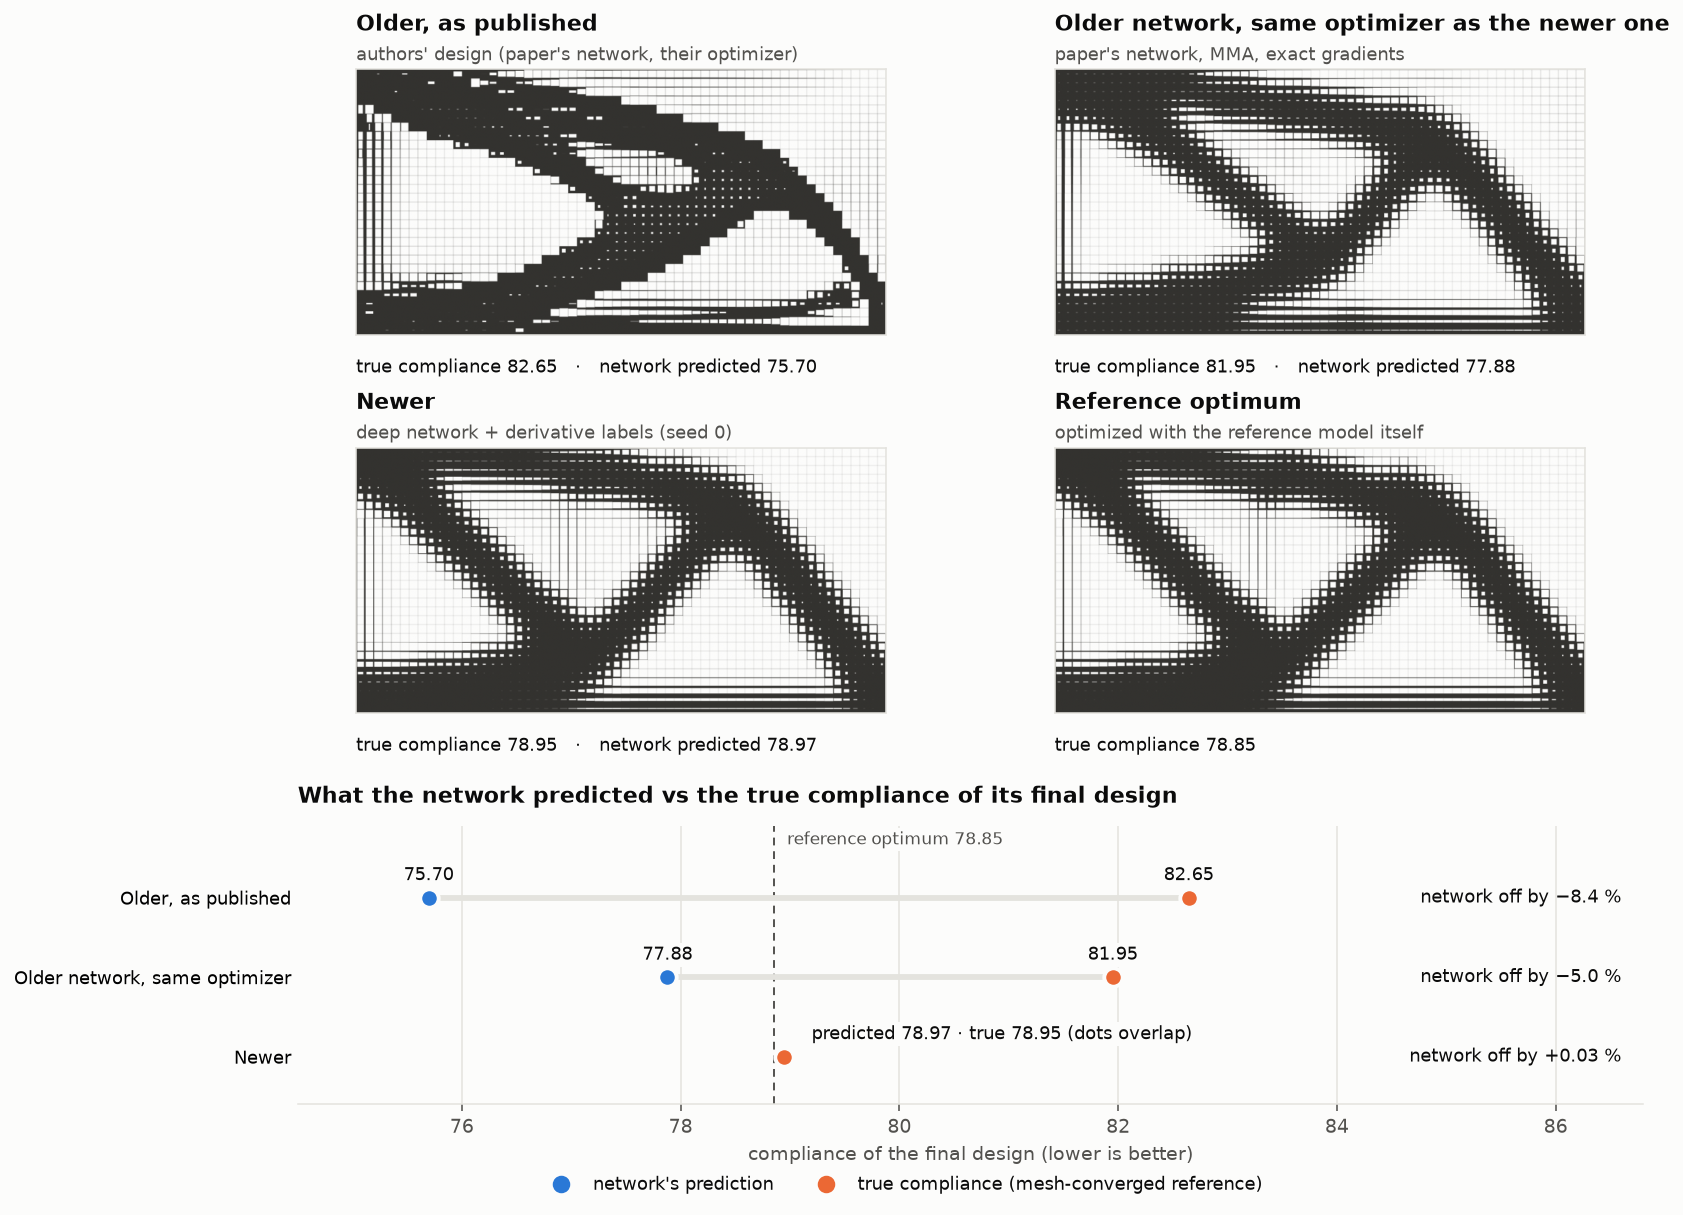
\includegraphics[width=\linewidth]{figures/fig5_older_vs_newer.png}
\caption{Top: final HBTO designs of the authors (published network, their
optimizer), of the published network with the formulation and optimizer of
Section~\ref{sec:extra}, of the 3$\times$64 tanh MLP trained on converged data
with derivative labels (seed 0), and of the reference model. Bottom: the
compliance each network predicts for its own final design and the true
compliance of that design.}
\label{fig:designs}
\end{figure}

\subsubsection{Limitations} The improved networks were trained on different data
(2\,601 converged samples with derivatives instead of the 7\,000 voxel training
rows of the original study). Filter and optimizer were changed together, so
their effects are not separated. Each configuration has two or three runs, and
only the $60\times30$ half MBB beam was studied. Derivative-informed (Sobolev)
training of surrogates for multiscale optimization has been used
before\supercite{White:2019}, and network derivatives have been compared with
finite-element sensitivities\supercite{Black:2023}; the contribution here is an
end-to-end ranking of the sources of error on the original benchmark, checked
against a converged reference.

\FloatBarrier
\section{Discussion}

\subsubsection{Was the replication successful?} Yes, in the sense of computational
replication: an independent implementation reproduces every result of the
original article that can be recomputed from the released material, and the
authors' own code reproduces their saved numbers. Three of the four
conclusions, however, do not hold once checks that the original study did not
make are added: a comparison in double precision, repeated optimization runs,
and a reference model for the HBTO problem. We therefore consider this a
successful replication of the computations, with revised conclusions.

\subsubsection{What was easy} The authors published their trained networks, their
data set and the result files of every run, including the initial
sensitivities and the final designs. This made it possible to compare our
numbers with theirs to many digits and to trace the CFD discrepancy to its
cause.

\subsubsection{What was difficult} The optimization scripts need TensorFlow and
start running when imported; according to the authors' logs, each HBTO run
with their optimizer takes 30--36 hours, mostly in dense linear algebra; the
article and the code differ in several places
(Table~\ref{tab:discrepancies}); the DBTO optimization paths are chaotic, so
single runs cannot be matched; and the original study offers no reference for
the HBTO problem, which we had to build.

\subsubsection{Recommendations} For comparisons of derivative methods inside an
optimization loop we suggest (1) running every method in double precision and
checking the precision that the framework actually uses; (2) scoring the final
designs with a model independent of the network that produced them;
(3) repeating runs with small perturbations to obtain a noise floor before
ranking methods; and (4) giving the optimizer a gradient consistent with the
objective it evaluates. These points agree with existing guidance on
benchmarking and replication in topology
optimization\supercite{Sigmund:2022,Haftka:2019} and on the use of neural
networks in it\supercite{Woldseth:2022}.

\section{Conclusion}
The computations of Najmon and Tovar\supercite{Najmon:2024} replicate, and
their first conclusion holds: the analytic network Jacobian, the complex step
and automatic differentiation give the same derivatives of a smooth network.
Their finite-difference discrepancy is a single-precision artefact, their
ranking of methods in density-based optimization is within the noise of single
runs, and in homogenization-based optimization the accuracy of the network,
not the choice of derivative method, determines the quality of the designs.
With a network trained on converged data with derivative labels, the designs
come within 0.12\,\% of the optimum obtained with the reference model.

\section*{Acknowledgements}
We thank J.~Najmon and A.~Tovar for publishing their code, trained networks,
data and results, without which this replication would not have been possible.
This work received no specific funding.

\subsubsection{Use of AI tools} The author designed and directed this study and
ran the complete replication package independently on his own computer. He used
an AI assistant (Claude, Anthropic) throughout the work: to audit the original
article and code, to write most of the replication code (the NumPy/SciPy
implementation, the reference models, the experiment scripts and the unit
tests), to run and re-run experiments, and to draft and edit this manuscript and
check its numbers against the result files. The author takes full
responsibility for the content.
